\chapter{Future Work: Application Characterization and Combined Modeling}
\label{ch:future}

\section{Measuring Additional Communication Capabilities}

The microbenchmarks presented in Chapters~\ref{ch:explicit}~and~\ref{ch:unified} cover CUDA transfers with the unified memory system and \texttt{cudaMemcpy}.
There are two additional CUDA communication capabilities that are not measured in this thesis: direct peer access and system atomics.
Expanding the benchmarks to measure those methods would provide a more complete view of CUDA communication performance.
THe benchmarks could also be expanded to examine interaction between CUDA and other system components.
One such opportunity is the GPUDirect capability, where supported non-GPU devices can communicate with CUDA GPUs through DMA.
Another opportunity is to investigate the effect of contention on the communication performance.
Such contention could occur in bi-directional data transfers, or when multiple devices are simultaneously communicating.

\section{Mapping Logical Communication to Underlying Links}
\label{sec:map-underlying}

Previous sections described the approach and results of measuring the data transfer performance of the logical communication paths.
Those models took some knowledge of the underlying system configuration as \textit{a priori} knowledge, but in general this process should be automated.
Application developers who want to understand the performance of the system may not have the architecture background to select appropriate performance models.
System architects who develop system capabilities may not understand the implications their choices have on performance at the top abstraction layer.
This work presents an initial step towards automation with automatic hardware enumeration described in Section~\ref{sec:hardware-enumeration}.

The next step is to systematically instrument all possible links for observation during the execution of applications.
If the instrumentation is low-overhead, this could be done jointly with logical performance measurements.
If not, known, separate workloads could be sent over logical communication paths to observe hardware links.
For NVLink monitoring, NVML provides the ability to query the link utilization counters~\cite{nvidia2017nvmlreference}.
For PCIe monitoring, the Performance Counter Monitor~\cite{opcm2018pcm} project provides the ability to query PCIe link counters.

For each enumerated link, the utilized hardware components could be associated and used to select the appropriate performance model.
Follow-up work investigating the feasibility of using a single parameterized model per combination of logical communication path and hardware link.
For example, consider a simple model to compute the transfer time $t_{transfer}$ for moving $bytes$ bytes between some CPU and GPU

\[
    t_{transfer} = c + t_{bytes}
\]

where $t_{bytes}$ is defined as

\[ \begin{cases} 
    max(BW_{link}, \frac{bytes}{BW_{L1}}) & 0 \leq bytes < L1_{size} \\
    max(BW_{link}, \frac{bytes}{BW_{L2}}) & L1_{size} \leq bytes < L2_{size} \\
    max(BW_{link}, \frac{bytes}{BW_{L3}}) & L2_{size} \leq bytes < L3_{size} \\
    max(BW_{link}, \frac{bytes}{BW_{mem}}) & L3_{size} \leq bytes  \\
 \end{cases}
\]

and $c$, $BW_{link}$, $BW_{L1}$, $BW_{L2}$, $BW_{L3}$, $BW_{mem}$ are some constant overhead, and the bandwidth of the CPU-GPU link, the L1 cache, L2 cache, L3 cache, and main memory.

In this model, the bandwidth is a piecewise function that depends on the transfer size - if a transfer fits within a cache, it happens at the speed of that cache.
In all cases, the transfer never happens faster than the underlying CPU-GPU link bandwidth.
The empirical results from the benchmark can be used to determine the constants in this model.

\section{Application Model}
\label{sec:app-model}

After a model of system communication performance is established, the next step is to establish an understanding of how applications use the logical communication paths.
This would encapsulate information about how an application produces, moves, and consumes data.
The application can be modeled as a dynamic value dependence graph (DVDG) $G_a = \{E_a,V_a\}$ where $E_a$ is a set edges representing data transfer, and $V_a$ is a set of vertices representing data values.
Each value represents a contiguous region of memory that the program interacts with.
Each edge is either an explicit memory copy or a CUDA kernel launch.
The edges can be tagged with observed timestamps to facilitate program performance analysis.

Table~\ref{tab:dvdg} shows an example code and corresponding DVDG.
Each value, represented by square boxes, is tagged with the position of the value, and size of the value.
For simplicity's sake, it is also tagged with the line of code that produced it.
Each rounded-box edge label corresponds to the \texttt{cudaMemcpy} or kernel execution.
In practice, each node and edge would have much more detailed information.

\begin{table}[ht]
	\centering
    \caption[Dynamic Value Dependence Graph]{
        Example of the dynamic value dependence graph for a simple vector add.
        Allocations in the code are commented with a hypothetical position of the allocation.
        Square blocks represent values, and rounded boxes represent node labels.
    }
    \label{tab:dvdg}
    \begin{tabular}{c}
        \begin{minipage}{\textwidth}
            \begin{lstlisting}
 1. float *a_h, *b_h, *s_h, *a_d, *b_d, *s_d;
 2. malloc(a_h, 1024);      // a_h = 0x0000
 3. malloc(b_h, 1024);      // b_h = 0x0400
 4. malloc(s_h, 1024);      // s_h = 0x0800
 5. cudaMalloc(&a_d, 1024); // a_d = 0x0c00  
 6. cudaMalloc(&b_d, 1024); // b_d = 0x1000
 7. cudaMalloc(&s_d, 1024); // s_d = 0x1400
 8. cudaMemcpy(a_d, a_h, 1024, cudaMemcpyDefault);
 9. cudaMemcpy(b_d, b_h, 1024, cudaMemcpyDefault);
10. vector_add<<<gd, bb>>>(s_d, a_d, b_d, 1024);
11. cudaMemcpy(s_h, s_d, 1024, cudaMemcpyDefault);
            \end{lstlisting}
        \end{minipage}        
    \\
        \begin{minipage}{\textwidth}
            \centering
            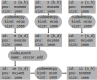
\includegraphics[width=0.5\textwidth]{figures/generated/dvdg.pdf}

        \end{minipage}

	\end{tabular}
\end{table}

Though it is generally possible to generate these dependence graphs by hand, it is not feasible for complicated applications.
Furthermore, as applications are updated, new models would have to be manually generated.
The proposed method described in this section would automate that process.

\section{Constructing the Dynamic Value Dependence Graph for Unmodified Applications}

Ideally, the DVDG would be generated from an unmodified application execution.
This ensures that the tool is as accessible to users as possible, and that it can work on closed-source applications
Unfortunately, the DVDG cannot rely on the application to advertise any helpful information about its behavior, and any relevant application state must be observed through its interaction with the operating system.
The proposed system (``apptracer'') leverages two tools available on the Linux platform: the CUDA Profiling Tools Interface (Section~\ref{sec:cupti} (CUPTI) and the Linux \texttt{LD\_PRELOAD} (Section~\ref{sec:ldpreload}) mechanism.

\texttt{apptracer} would use CUPTI to capture most CUDA-related information, and LD\_PRELOAD for everything else.
CUPTI allows a tool to provide a callback function that is invoked at every CUDA runtime or driver call, and also allows \texttt{apptracer} to collect any performance metrics the GPU exposes.
The callback function records relevant information, including the wall time when the CUDA runtime function is invoked, its arguments, and the device and stream associated with the call.
In this way, detailed information about data transfers from runtime functions can be reconstructed.
For example, allocations from \texttt{cudaMalloc} can be associated with pointers passed to \texttt{cudaMemcpy} to discover data transfers from host to device.

\texttt{apptracer} would use \texttt{LD\_PRELOAD} (Section~\ref{sec:ldpreload}) to intercept known API calls made by the application to shared libraries.
For example, \texttt{LD\_PRELOAD} could be used to observe file access, calls to CUDA libraries such as cuDNN or cuBLAS, network access, and system memory allocations.
The various kernel launches and allocations used by cuDNN and cuBLAS are already visible through CUPTI, but the known semantics of the higher-level cuBLAS and cuDNN calls allow for detailed edges to be added.

One challenge of \texttt{apptracer} is handling implicit data movement from three scenarios:
data moved from GPU global memory to arbitrary GPU kernels, implicit data movement between remote mappings, and implicit data movement through the unified memory system.
On supported systems, GPUs can directly access data that is on the host or other GPUs without making any CUDA runtime calls.
CUPTI allows the GPU to record detailed profiling information, but this affects program execution time and distorts the timeline.
A two-pass approach, once to collect accurate timeline information and another to capture more detailed information may be a solution.

Another challenge is for \texttt{apptracer} to infer which kernel arguments are pointers to allocations.
It may be possible for \texttt{apptracer} to examine the intermediate PTX representation of CUDA kernel code embedded in most CUDA binaries, and deduce some information about function signatures.

Once the application's use of CUDA is recorded, the next step would be to extend the graph to some view of activity on the CPU as well.
This could be accomplished through a variety of techniques.
The \texttt{LD\_PRELOAD} mechanism could be used to instrument popular libraries such as BLAS or MPI.
The operating system trace facilities strace~\cite{strace2018} for Linux, DTrace~\cite{dtrace2008} for MacOS, NtTrace~\cite{orr2014nttrace}, or Dr. Memory~\cite{bruening2001design}\cite{drmemory2018} for Windows could be used to track system calls and profile things such as file I/O or network interaction.
Tracking arbitrary function calls within an unmodified application may not be possible in the case of a binary without debug symbols.
Dynamic tracing tools like Intel's PIN~\cite{intel2012pin} can insert instrumentation code, but further work would be needed to determine the number of function arguments and their locations to recover their values.
For a cluster environment, it may be possible to generate distributed dependence graphs at each node, and then join them together by linking together information recorded about MPI calls.

\section{Combined Modeling}
\label{sec:modeling}

Finally, once system performance modeling is established, and application demands are recorded, joint performance modeling is possible, to tackle questions like
\begin{itemize}
    \item For a particular DVDG, what performance could we expect on a particular system?
    \item For a particular DVDG and a particular budget, what system configuration would perform best?
    \item For a particular DVDG, can the execution be rescheduled on a system to improve performance?
    \item How would changing link parameters or topology on a particular system affect application performance?
\end{itemize}
Answering these questions may require additional effort in open research challenges, such as task scheduling with placement-dependent communication costs, compute kernel performance estimation, and design space exploration.
